\newcommand{\booktitle}{User Manual}
\newcommand{\tocname}{Contents}
\newcommand{\chapword}{Chapter \thesection}
\documentclass[11pt,a4paper]{article}
\usepackage[top=20mm,bottom=21mm,left=22mm,right=22mm,headheight=16pt,footskip=11mm]{geometry}
\usepackage{fontspec,xeCJK,graphicx,xcolor,tabularx,array,booktabs,enumitem,fancyhdr,hyperref}
\setmainfont{TeX Gyre Pagella}
\setsansfont{TeX Gyre Heros}
\setmonofont[Scale=.89]{Latin Modern Mono}
\IfFileExists{C:/Windows/Fonts/msyh.ttc}
{\setCJKmainfont[AutoFakeBold=2]{SimSun}\setCJKsansfont{Microsoft YaHei}\setCJKmonofont{Microsoft YaHei}}
{\setCJKmainfont[BoldFont=FandolSong-Bold.otf]{FandolSong-Regular.otf}\setCJKsansfont[BoldFont=FandolHei-Bold.otf]{FandolHei-Regular.otf}\setCJKmonofont{FandolHei-Regular.otf}}
\definecolor{ink}{HTML}{18373A}\definecolor{teal}{HTML}{006B64}
\definecolor{muted}{HTML}{496164}\definecolor{wash}{HTML}{EAF4F0}\definecolor{linecolor}{HTML}{A3C0B6}
\hypersetup{unicode=true,colorlinks=true,linkcolor=teal,urlcolor=teal,bookmarksnumbered=true,pdftitle={IM Tool — \booktitle},pdfauthor={IM Tool}}
\setlength{\parindent}{0pt}\setlength{\parskip}{6pt}\linespread{1.09}
\setlist[enumerate]{leftmargin=1.85em,itemsep=3pt,topsep=2pt,parsep=0pt,label=\textcolor{teal}{\sffamily\bfseries\arabic*.}}
\raggedbottom\setlength{\emergencystretch}{2em}
\pagestyle{fancy}\fancyhf{}\fancyhead[L]{\sffamily\bfseries\color{teal} IM Tool}
\fancyhead[R]{\small\sffamily\color{muted}\nouppercase{\leftmark}}
\fancyfoot[L]{\footnotesize\sffamily\color{muted}\booktitle\enspace ·\enspace 1.2.4}
\fancyfoot[R]{\sffamily\bfseries\color{teal}\thepage}
\renewcommand{\headrule}{{\color{linecolor}\hrule height .65pt width\headwidth}}
\renewcommand{\contentsname}{\tocname}
\newcommand{\code}[1]{{\ttfamily\detokenize{#1}}}
\newcommand{\ui}[1]{{\sffamily\bfseries\color{ink}#1}}
\newcommand{\chapterpage}[2]{\clearpage\refstepcounter{section}\label{#1}\markboth{#2}{}%
\addcontentsline{toc}{section}{\protect\numberline{\thesection}#2}%
{\sffamily\bfseries\color{teal}\chapword\par}\vspace{1mm}%
{\raggedright\sffamily\bfseries\fontsize{23}{29}\selectfont\color{ink}#2\par}\vspace{2mm}}
\newcommand{\subhead}[1]{\par\addvspace{2mm}{\large\sffamily\bfseries\color{teal}#1\par}\nobreak}
\newcommand{\note}[2]{\par\smallskip\colorbox{wash}{\parbox{\dimexpr\linewidth-2\fboxsep\relax}{\raggedright\vspace{1mm}\sffamily\textbf{\color{teal}#1}\enspace#2\vspace{1mm}}}\par}
\newcommand{\tbl}[3]{\par\smallskip\begingroup\small\renewcommand{\arraystretch}{1.23}
\begin{tabularx}{\linewidth}{@{}>{\raggedright\arraybackslash}p{.30\linewidth}>{\raggedright\arraybackslash}X@{}}
\toprule\sffamily\bfseries\color{teal}#1&\sffamily\bfseries\color{teal}#2\\\midrule #3\bottomrule\end{tabularx}\endgroup\par}
\newcommand{\pic}[3]{\par\smallskip\begingroup\centering\includegraphics[width=\linewidth,height=#3,keepaspectratio]{figures/#1.png}\par\endgroup{\small\color{muted}#2\par}\smallskip}
\newcommand{\cover}[3]{\thispagestyle{empty}\vspace*{12mm}
\includegraphics[width=29mm]{../../im_app/resources/im-tool.png}\par\vspace{12mm}
{\sffamily\bfseries\fontsize{50}{54}\selectfont\color{ink}IM Tool\par}\vspace{3mm}
{\sffamily\bfseries\fontsize{28}{34}\selectfont\color{teal}\booktitle\par}\vspace{4mm}
{\Large\color{muted}#1\par}\vfill
\begin{flushleft}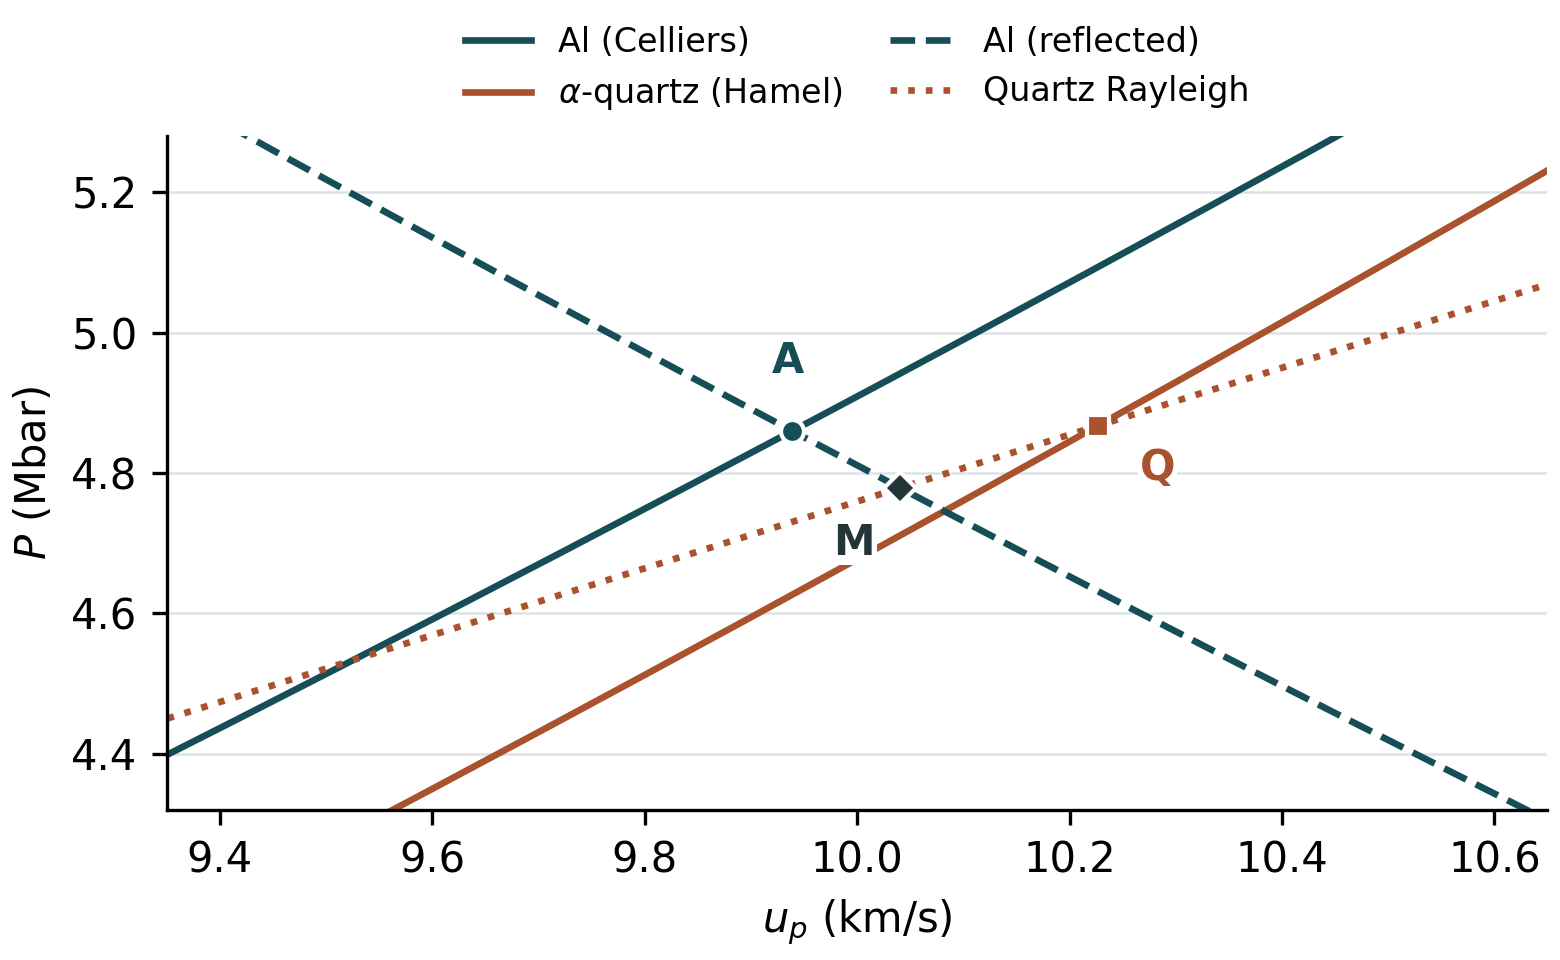
\includegraphics[width=.67\linewidth,height=81mm,keepaspectratio]{figures/tutorial-plot.png}\end{flushleft}
{\small\color{muted}#2\par}\vfill{\color{linecolor}\rule{\linewidth}{.7pt}}\par
{\large\sffamily\bfseries\color{ink}#3}\hfill{\sffamily\color{muted}2026.11}\clearpage}

\begin{document}\color{ink}
\cover{Impedance matching and material data visualization}{Hicks shot 29400. A and Q locate the measured shock speeds on the Celliers aluminum and Hamel quartz fits. M is the quartz interface estimate from the reflected aluminum Hugoniot and the quartz Rayleigh line.}{Desktop edition 1.2.4\enspace ·\enspace Bo Xu}
\phantomsection\pdfbookmark[1]{Contents}{contents}\markboth{Contents}{}\tableofcontents
\subhead{Your first session}
Choose \ui{Help → Open Practice Workspace}. Chapters~\ref{workspace} and~\ref{crossing} use two measured shock speeds from Hicks shot 29400 to compare the Celliers aluminum and Hamel quartz standards and estimate the interface pressure. The equations and sources are on page~\pageref{sources}.
\note{Interface language}{Both manuals use the application's English control names. The Windows installer also offers Simplified Chinese. The installation screenshot shows the Windows wizard. The data-analysis screenshots show the Qt application on Ubuntu.}

\chapterpage{windows}{Install on Windows}
\begin{enumerate}
\item On 64-bit Windows 10 or 11, double-click \code{IM-Tool-Setup-1.2.4-x64.exe}. Choose English or Simplified Chinese for the installation wizard.
\item Choose the installation folder. The default for your account is\\
\verb|%LOCALAPPDATA%\Programs\IM Tool|. The installer includes Python, Qt and the plotting libraries.
\item Choose whether to create a desktop shortcut, then select \ui{Install}. On the final page, leave \ui{Launch IM Tool} selected to open the application immediately, or start \ui{IM Tool} from the Start menu later.
\item Open \ui{Help}. Choose either manual to open a local PDF with your default reader. Choose \ui{Open Practice Workspace} to begin the exercise.
\end{enumerate}
\pic{wizard-en}{The English welcome page. Select Next to choose the installation folder and desktop shortcut.}{77mm}
\subhead{Where your work goes}
The first desktop launch copies the starter material library into your profile. \ui{Help → Open Working Folder} shows the active \code{standard_library} directory. Its sibling \code{workflows} folder is the default save location for JSON sessions. The aluminum and quartz exercise has its own library and workflows under \code{Practice/Celliers-Hamel}.
\subhead{Updating or removing the application}
Close running IM Tool windows before running a newer installer. Use the existing destination to update the application and its bundled manuals. An existing user library is reused, including the tables you added. To remove the program, open \ui{Settings → Apps → Installed apps} and choose \ui{Uninstall}. Your working files are stored in your user profile and can be backed up independently.
\note{First-launch check}{Look for the crossed-curve icon, the nine diagram tabs and the Help menu. A blank plot is normal until you select a material.}

\chapterpage{linux}{Install on Linux}
Choose the package for your distribution. In a graphical file manager, open the local package with the system software installer, review its dependencies, then install it. If double-click opens an archive viewer, use \ui{Open With} and choose the software installer, or run the corresponding command below from the folder containing the download.
\tbl{Distribution}{Package and command}{
Debian or Ubuntu & \code{im-tool_1.2.4-1_all.deb}\\[-1pt]
& \code{sudo apt install ./im-tool_1.2.4-1_all.deb}\\
Fedora & \code{im-tool-1.2.4-1.noarch.rpm}\\[-1pt]
& \code{sudo dnf install ./im-tool-1.2.4-1.noarch.rpm}\\}
The desktop packages use the distribution's Python 3, PyQt5, plotting libraries and spreadsheet readers. Package installation can require access to the distribution repositories. Once installed, the application, manuals and practice tables work offline.
\subhead{Launch and verify}
In your desktop session, search the applications menu for \ui{IM Tool}. Alternatively run \code{im-tool} from a terminal. If the program exits at startup, that terminal displays the first error. The Qt application needs a graphical session. A remote text shell alone cannot display the window.
\subhead{Find files, update or uninstall}
The installed application resources are under \code{/usr/share/im-tool/}. The default user data location is \verb|~/.local/share/IM Tool/|, or the corresponding directory under \code{XDG_DATA_HOME}. Use \ui{Help → Open Working Folder} to see the active library. To update, install the newer local package with the same package manager. For a rebuilt package with the same version, use \code{apt reinstall} or \code{dnf reinstall} with the local package path. Use \code{sudo apt remove im-tool} or \code{sudo dnf remove im-tool} to uninstall.
\note{Which version is installed?}{On Ubuntu or Debian run \code{dpkg-query -W im-tool}. On Fedora run \code{rpm -q im-tool}. Start the GUI as your normal user so newly created files belong to you.}

\chapterpage{macos}{Install on macOS}
In the Apple menu, choose \ui{About This Mac}. Use the \code{arm64} disk image if the Chip field names an Apple M-series chip. Use the \code{x86_64} image if the Processor field names Intel. The application includes Python, Qt, the starter tables and both offline manuals.
\tbl{Mac}{Disk image for version 1.2.4}{
Apple silicon & \code{IM-Tool-1.2.4-macOS-arm64.dmg}\\
Intel & \code{IM-Tool-1.2.4-macOS-x86_64.dmg}\\}
\begin{enumerate}
\item Double-click the disk image in Finder. Drag \ui{IM Tool.app} onto the \ui{Applications} shortcut in the window and wait for the copy to finish.
\item Eject the \ui{IM Tool} disk image in Finder. Open \ui{Applications} and double-click \ui{IM Tool}.
\item Choose \ui{Help → Open Practice Workspace}. The exercise opens with the Celliers aluminum and Hamel quartz standards. Choose either manual in \ui{Help} to open the bundled PDF.
\end{enumerate}
\subhead{If macOS asks for approval}
This release uses an ad hoc signature and has no Apple notarization. If Gatekeeper blocks the first launch, verify the download source. For a copy you trust, follow the per-app approval in \ui{System Settings → Privacy \& Security → Open Anyway}. \href{https://support.apple.com/en-us/102445}{Apple's first-launch instructions}.
\subhead{Work files, updates and removal}
Your writable library is under \verb|~/Library/Application Support/|. Use \ui{Help → Open Working Folder} to locate the active library and its sibling \code{workflows} folder. To update, quit the application, drag the newer copy to Applications and choose \ui{Replace}. To uninstall, move \ui{IM Tool.app} from Applications to the Trash. Your work is stored separately in your account.

\chapterpage{workspace}{Load the two reference materials}
Open \ui{Help → Open Practice Workspace}. The new window selects \ui{Aluminum} (\code{Al_Celliers2005}) and \ui{Alpha Quartz} (\code{Quartz_Hamel2012}) from the standard library. Each table samples a published fit at 500 velocities.
\begin{enumerate}
\item In \ui{Rayleigh Lines}, check the two preloaded shock speeds from Hicks et al., Table I, shot 29400. Aluminum has $D=18.11\pm0.32$ km/s and $\rho_0=2.70$ g/cm³. Quartz has $D=17.96\pm0.26$ km/s and $\rho_0=2.65$ g/cm³. Double-click a line to inspect its values.
\item In \ui{Find Intersection}, choose \ui{Aluminum} and its \ui{Rayleigh} entry ($D=18.11$). Click \ui{Find Intersection}. This gives the aluminum starting state A, with $u_p=9.9390$ km/s and $P=4.8599$ Mbar.
\item Repeat with \ui{Alpha Quartz} and the quartz \ui{Rayleigh} entry ($D=17.96$). The Hamel fit gives state Q at 10.2267 km/s and 4.8673 Mbar. Keep both rows for the next chapter.
\end{enumerate}
\pic{workspace}{The exercise opens with the two fitted Hugoniots and both measured-speed lines in the pressure range of shot 29400.}{78mm}
\note{Identify the rows}{This manual calls the three results A, Q and M in calculation order. The application assigns its own intersection IDs. Open \ui{Help → Open Working Folder} to inspect the two material files.}

\chapterpage{crossing}{Match aluminum to quartz}
\begin{enumerate}
\item In \ui{Reflect / Release}, set \ui{Curve} to \ui{Aluminum}. In \ui{About intersection}, choose the aluminum row A from Chapter~\ref{workspace} ($u_p=9.9390$ km/s). Click \ui{Reflect} to mirror the Celliers curve about that particle velocity.
\item Set \ui{Curve 1} to \code{Reflected Al_Celliers2005}. For \ui{Curve 2}, select the quartz Rayleigh line ($D=17.96$). Click \ui{Find Intersection}. The new row M gives $u_p=10.0405$ km/s and $P=4.7787$ Mbar (477.87 GPa).
\item Compare M with the value inferred in Hicks Table I, 4.79 Mbar at 10.07 km/s. The authors give random and systematic pressure uncertainties of 0.17 and 0.04 Mbar. Q (4.8673 Mbar) is a separate estimate using the Hamel quartz fit and measured quartz speed.
\end{enumerate}
\pic{intersection}{The selected third row uses reflected aluminum and the quartz Rayleigh line. The first two rows identify the states on the principal Hugoniots.}{76mm}
\subhead{What the construction assumes}
IM Tool mirrors each aluminum point as $u_p'=2u_{p,A}-u_p$ at fixed $P$. This approximates the aluminum release path. The quartz line obeys $P\,(\mathrm{Mbar})=0.01\rho_0 D u_p$ when density is in g/cm³ and both velocities are in km/s.
\note{Compare like quantities}{The experimental inputs are the two shock speeds. Both the published interface pressure and the value reconstructed here depend on the material model and release treatment.}

\chapterpage{sources}{Reference fits and experimental inputs}
\textbf{Celliers aluminum.} With speeds in km/s and $\rho_0=2.70$ g/cm³, the standard library uses
\[
 U_s=17.992+1.167(u_p-9.838).
\]
The 500 stored rows sample $u_p=0$ to 50 km/s. The header gives the fit coefficients and their uncertainties. \href{https://doi.org/10.1063/1.2140077}{Celliers et al., J. Appl. Phys. 98, 113529 (2005).}

\textbf{Hamel alpha quartz.} With $\rho_0=2.65$ g/cm³, the library evaluates the quadratic below 15 km/s and continues along its tangent above the join. The 500 rows span 0.1 to 50 km/s.
\[
\begin{array}{ll}
U_s=2.40+1.68u_p-0.0155u_p^2 & (u_p<15),\\
U_s=5.8875+1.215u_p & (u_p\geq15).
\end{array}
\]
The quartz reference fit is given in Hamel's study of CH$_{1.36}$. The sampling grid in each file describes its coverage. For use outside this example, consult the calibration data in the publications. \href{https://doi.org/10.1103/PhysRevB.86.094113}{Hamel et al., Phys. Rev. B 86, 094113 (2012).}

\subhead{Where the measured speeds come from}
Table I of Hicks et al. lists shot 29400 with $U_s^{\rm Al}=18.11\pm0.32$ and $U_s^{\rm Q}=17.96\pm0.26$ µm/ns. Numerically, 1 µm/ns equals 1 km/s. The paper infers $P^{\rm Q}=4.79$ Mbar, $\rho^{\rm Q}=6.03$ g/cm³ and $u_p^{\rm Q}=10.07$ km/s using its aluminum standard. The exercise uses only the two speeds as experimental inputs. \href{https://doi.org/10.1063/1.2009528}{Hicks et al., Phys. Plasmas 12, 082702 (2005), Table I.}

\subhead{Check the units independently}
At $u_p=10.0$ km/s the Hamel table gives $U_s=17.65$ km/s. The stored pressure is $0.01\times2.65\times17.65\times10=4.67725$ Mbar. For aluminum the analytical fit at the same $u_p$ gives 4.90888 Mbar. Linear interpolation in the sampled aluminum table gives 4.90894 Mbar.

\chapterpage{materials}{Read and validate a material table}
The desktop starter library includes aluminum, quartz, boron nitride, diamond, copper and lithium fluoride tables. Search by material name, ID, source or tag. The checkboxes select curves for plotting. When the search field is active, \ui{Select All} and \ui{Deselect All} apply to the visible results.
\subhead{Read a standard table}
Open \code{materials/Quartz_Hamel2012.txt} or \code{materials/Al_Celliers2005.txt} in the practice library. Each UTF-8 file contains tab-separated columns. The comment header documents the fit, the coefficients used for uncertainty propagation and the initial density.
\tbl{Column}{Meaning and unit}{
\code{Up(km/s)}, \code{Us(km/s)} & Particle velocity and shock velocity in kilometres per second.\\
\code{P(Mbar)} & Pressure. At $u_p=10.0$ km/s the Hamel table contains 4.67725 Mbar (467.725 GPa).\\
\code{rho(g/cm3)}, \code{compression} & Density in g/cm³ and dimensionless density ratio. These complete the five required columns.\\
\code{T(eV)}, \code{E(MJ/g)} & Optional temperature and specific internal energy. These columns have no values in either fit table.\\}
\subhead{Check a file before adding it}
Select \ui{Validate File}, then \ui{Browse}, select the practice table and click \ui{Validate}. Read the record count, column information, errors and warnings. A successful check confirms that the file meets the validator's tests. Review its provenance, units and physical interpretation separately.
\subhead{Add your own table}
\ui{Add New Material} guides you through material information, data input and review. Supply an identifiable name, source and initial density. Paste tabular data or use \ui{Import from File}. Check the preview and output filename before finishing. After saving, use \ui{Refresh}, then search for the new entry. Keep the original input for traceability.

\chapterpage{validation}{Check an imported table}
\begin{enumerate}
\item In the practice window choose \ui{Help → Open Working Folder}. Open the \code{materials} folder and select \code{Quartz_Hamel2012.txt}. Its header gives the fit, the 15 km/s join and the initial density.
\item Under \ui{Material Library} choose \ui{Validate File}, then \ui{Browse} and \ui{Validate}. The quartz file has 500 rows and no warnings. Repeat for \code{Al_Celliers2005.txt}. It also has 500 rows.
\item Read the quartz row at $u_p=10.0$ km/s. It gives $U_s=17.65$ km/s, $P=4.67725$ Mbar, $\rho=6.11405$ g/cm³ and a compression ratio of 2.30719. This row samples the fit independently of shot 29400.
\end{enumerate}
\pic{validation}{The validator reports the Hamel quartz file's 500 rows, initial density and ranges. The 500 values are samples of its fitted curve.}{78mm}
\subhead{Common import errors}
If columns collapse into one field, open the file in a text editor and check for tabs between names and values. If a column is reported missing, match the spelling and unit in the header to the list on page~\pageref{materials}. If the curve looks wrong, compare several original rows and the stated initial density before changing its display range.
\note{Keeping comparable versions}{For a revised table, use a distinct material ID or keep a versioned copy of the old library. A workflow refers to material IDs, so replacing values under the same ID can change a later replay.}

\chapterpage{views}{Read the nine diagram tabs}
The default axes below were checked in the running desktop application. Some tab names put the vertical variable first and some put it second. Read the axis captions whenever you switch tabs or invert the axes.
\tbl{Diagram}{Default horizontal axis → vertical axis}{
P-Up & Particle velocity (km/s) → pressure (Mbar). Main view for matching curves and selecting intersections.\\
P-CR & Compression ratio → pressure (Mbar).\\
P-rho & Density (g/cm³) → pressure (Mbar).\\
Us-Up & Shock velocity (km/s) → particle velocity (km/s).\\
P-T & Pressure (Mbar) → temperature (eV).\\
rho-Up & Density (g/cm³) → particle velocity (km/s).\\
T-Up & Temperature (eV) → particle velocity (km/s).\\
E-Up & Internal energy (MJ/g) → particle velocity (km/s).\\
P-Us & Pressure (Mbar) → shock velocity (km/s).\\}
\subhead{Adjust one plot}
Choose the diagram under \ui{Target Plot} and inspect the axis descriptions. Set limits, line width, legend or pressure unit, then press \ui{Apply}. Some controls are available only on the diagrams to which they apply. \ui{Inverse Axes} exchanges the coordinates on generic diagrams. Keep a copy of the axis labels and units with the exported image.
\subhead{Use the cursor and zoom}
Move the pointer inside the axes to read its coordinates in the status bar. Drag a rectangle to zoom. Focus the plot and press \ui{A} to fit the data again. A pointer position between samples is a coordinate reading. The intersection table records the numerical crossing calculated from the two selected curves.
\note{Pressure units}{1 Mbar equals 100 GPa. In the example, 4.7787 Mbar corresponds to 477.87 GPa. The two fits supply no temperature or energy trace on the P-T, T-Up and E-Up tabs.}

\chapterpage{controls}{Set a view and place a marker}
\begin{enumerate}
\item Open \ui{P-rho Diagram} and set pressure to Mbar in \ui{Plot Settings}. For shot 29400, Hicks Table I gives an inferred quartz density of 6.03 g/cm³ and a pressure of 4.79 Mbar.
\item To see the experimental region clearly, set the density axis to 5.4–6.8 g/cm³ and the pressure axis to 3.5–6.3 Mbar. Click \ui{Apply}.
\item In the manual scatter inputs enter 6.030 and 4.790 and click \ui{Add}. This puts the paper's inferred state on the plot for comparison with the Hamel curve.
\end{enumerate}
\pic{settings}{The marker places the value reported by Hicks on the density–pressure diagram. Both reference fits are shown in the same units.}{88mm}
\subhead{Which type of mark should you save?}
For a value you read by eye, keep the tab, quantities and units with the manual point. For a computed crossing, select its ID in the scatter controls. IM Tool can use the associated state values on other diagrams when those values are available. Save the workflow to keep the marker list, and export a figure when a colleague only needs the visual result.

\chapterpage{tools}{Reference curves, markers and analysis controls}
\subhead{Overlay an independent reference}
Choose \ui{Reference Curves → Create New Curve}. Name the curve, select its variables, then type rows or use \ui{Load from File}. Inspect the preview and choose \ui{Save Curve}. Check the entry under \ui{Reference Curves} in the left column. The curve appears on diagrams for which it supplies the needed variables. \ui{Manage Curves} lists saved references. Keep a copy of a reference file before deleting or replacing it.
\subhead{Mark an intersection or a point you read}
The scatter controls accept a selected intersection or manual coordinates for the current tab. Check the displayed variable names and units before clicking \ui{Add}. A point created from an intersection carries the available state values to compatible diagrams. A manual point belongs to its chosen diagram. Use \ui{Delete Selected} if you need to correct it. Right-click a selectable plotted element to open its style controls.
\tbl{Other controls}{What the result represents}{
Rayleigh lines & A line constructed from the inputs shown in the panel. Select curve names explicitly when comparing it to a tabulated curve.\\
Reflect / Release & Overlays associated with a selected state or curve. Their labels distinguish a constructed curve from a loaded material table.\\
Reverse Match & Uses the chosen intersection and the selected reference. Recheck the named source objects after changing the plot.\\
Error bars and Monte Carlo & Display propagated uncertainty when estimates have been supplied. A missing uncertainty has a different meaning from a measured uncertainty of zero. Record the inputs and assumptions alongside the figure.\\}
\note{Separate values from display choices}{Changing a marker colour or the zoom level affects the figure. A new material selection, reference or intersection changes which data the analysis uses.}

\chapterpage{save}{Save figures and reopen a session}
\subhead{Save and reopen the exercise}
Use \ui{Save Workflow} in the practice window and save \code{hicks-29400-check.json} in its \code{workflows} folder. Restart IM Tool, open the practice window and use \ui{Load Workflow} to reopen your file. Check for both materials, two Rayleigh lines, one reflected aluminum curve and the three result rows, including M at 4.7787 Mbar.
A workflow stores material IDs, line definitions, intersections, reflected curves, scatter points and plot settings. The original tables live in the library. Keep their matching files and metadata when transferring a session. Reference overlays have separate files and may need to be selected again after loading. A JSON file can be reopened in a workspace that contains the required IDs.
\subhead{Export all diagrams}
Choose \ui{Save Plot} on the toolbar or \ui{File → Export Plot}. Select a new writable directory. Both actions write the nine PNGs below at the application's default export resolution of 300 dpi. The filenames are fixed, so use a new folder for each comparison.
\tbl{Diagram family}{Output filenames}{
Pressure views & \code{p_up_diagram.png}, \code{p_cr_diagram.png}, \code{p_rho_diagram.png}, \code{p_t_diagram.png}, \code{p_us_diagram.png}\\
Other views & \code{us_up_diagram.png}, \code{rho_up_diagram.png}, \code{t_up_diagram.png}, \code{e_up_diagram.png}\\}
\note{Handoff check}{Open the P-Up PNG and verify the axis units and selected curves. Reopen the JSON against the same material library to confirm the intersection. A PNG remains readable without the application.}

\chapterpage{trouble}{Troubleshoot a session}
\tbl{Symptom}{Checks to make}{
Installer opens as an archive & Use the distribution's software installer or the local APT/DNF command in Chapter~\ref{linux}. For a missing dependency, read the first package-manager error.\\
Program starts with an empty canvas & Check a material in the active window. Open the P-Up tab, focus the canvas and press \ui{A}. The practice window initially lists two tables.\\
A checked material is missing on one tab & Inspect the source columns for that tab's two quantities. Temperature and energy are optional. Check the selected axes and pressure unit.\\
Unexpected intersection & For A and Q, choose a material and its own measured-speed line. For the interface M, choose reflected aluminum and the quartz Rayleigh line. The crossing of the two principal Hugoniots alone does not incorporate either measured speed.\\
Library changes cannot be saved & Open the working folder from Help. Check the current user's write access and free space. For an installed desktop build, edit the user copy of a table.\\
Workflow opens with missing curves & Find the material IDs in the corresponding workspace and restore the matching files. Open \ui{Reference Curves} and reselect the intended overlays.\\
Offline manual does not open & Check the system's default PDF reader. On Linux the PDFs are under \code{/usr/share/im-tool/im_app/resources/manuals/}. On Windows look under \code{_internal/im_app/resources/manuals} in the installation folder.\\}
\subhead{Report a reproducible issue}
Include the platform, app version, diagram, material IDs and display units, or the practice steps that show the problem. For data issues, include the column names and a few representative rows you are able to share.
\end{document}
